\documentclass[10pt, aspectratio=169, handout]{beamer}
\usefonttheme{professionalfonts}

\mode<presentation>
{
  \usetheme{Berkeley}
  \usecolortheme{beaver}
  \usefonttheme{default}
  \setbeamertemplate{navigation symbols}{}
  \setbeamertemplate{caption}[numbered]
} 

\setbeamertemplate{footline}{%
  \leavevmode%
  \hbox{%
    \begin{beamercolorbox}[wd=.85\paperwidth,ht=2.5ex,dp=1ex,left]{author in head/foot}%
      \usebeamerfont{author in head/foot}Digital Signal Processing, Fall 2025%
    \end{beamercolorbox}%
    \begin{beamercolorbox}[wd=.15\paperwidth,ht=2.5ex,dp=1ex,right]{date in head/foot}%
      \hspace*{0.5em}\insertframenumber{} / \inserttotalframenumber\hspace*{0.5em}%
    \end{beamercolorbox}%
  }%
  \vskip0pt%
}

\usepackage[english]{babel}
\usepackage[utf8x]{inputenc}
\usepackage{tikz}
\usepackage{pgfplots}
\usepackage{array}
\usepackage{makecell}
\usepackage{verbatim}
\usepackage{graphicx}
\usepackage{subcaption}
\usepackage{amsfonts}
\usepackage{amsmath}
\usepackage{bm}
\usepackage{epstopdf}
\captionsetup{compatibility=false}

\usetikzlibrary{calc}
\usetikzlibrary{pgfplots.fillbetween, backgrounds}
\usetikzlibrary{positioning}
\usetikzlibrary{pgfplots.groupplots}
\usetikzlibrary{plotmarks}
\usetikzlibrary{calc}
\usetikzlibrary{patterns}
\usetikzlibrary{decorations.pathreplacing}

\usepgfplotslibrary{groupplots}
\pgfplotsset{compat=newest} 

\usepackage{ifthen}
\newboolean{showresults}
\setboolean{showresults}{false}

\usepackage{hyperref}
\hypersetup{
    colorlinks=true,
    linkcolor=blue,
    filecolor=magenta,      
    urlcolor=cyan,
}

\title[ECEN 463/863]{z-Transform Properties and LTI Systems}
\author{Maxx Seminario}
\institute{University of Nebraska-Lincoln}
\date{October 13, 2025}

\begin{document}
\begin{frame}
  \titlepage
\end{frame}

\section{Introduction}

\begin{frame}{Overview: z-Transform Properties}
\begin{itemize}
    \item \textbf{Motivation}: 
    \begin{itemize}
        \item Properties simplify analysis of discrete-time signals and systems
        \item Used with inverse z-transform techniques for complex expressions
        \item Foundation for solving difference equations algebraically
    \end{itemize}
    
    % \item \textbf{Notation}:
    % \begin{itemize}
    %     \item $x[n] \overset{\mathcal{Z}}{\longleftrightarrow} X(z), \quad \text{ROC} = R_x$
    %     \item $R_x$ represents: $r_R < |z| < r_L$
    %     \item For two sequences: $x_1[n] \overset{\mathcal{Z}}{\longleftrightarrow} X_1(z), \text{ROC} = R_{x_1}$ and $x_2[n] \overset{\mathcal{Z}}{\longleftrightarrow} X_2(z), \text{ROC} = R_{x_2}$
    % \end{itemize}
    
    \item \textbf{Applications}:
    \begin{itemize}
        \item Transform difference equations to algebraic equations
        \item Analyze LTI systems via system functions
        \item Compute convolutions efficiently
    \end{itemize}
\end{itemize}
\end{frame}

\section{Basic Properties}

\begin{frame}{Linearity}
\textbf{Property}: 
\[
ax_1[n] + bx_2[n] \overset{\mathcal{Z}}{\longleftrightarrow} aX_1(z) + bX_2(z), \quad \text{ROC contains } R_{x_1} \cap R_{x_2}
\]

\vspace{0.3cm}
\textbf{Key Points}:
\begin{itemize}
    \item ROC is at least the intersection of individual ROCs
    \item May be larger if pole-zero cancellation occurs
    \item Essential for partial fraction decomposition
\end{itemize}

\vspace{0.3cm}
\textbf{Example}: $x[n] = a^n(u[n] - u[n-N]) = a^n u[n] - a^n u[n-N]$
\begin{itemize}
    \item Both terms have pole at $z = a$ with ROC $|z| > |a|$
    \item Linear combination cancels pole $\Rightarrow$ ROC becomes entire z-plane (except $z = 0$)
    \item Infinite-duration components combine to finite-duration sequence
\end{itemize}
\end{frame}

\begin{frame}{Time Shifting}
\textbf{Property}: 
\[
x[n - n_0] \overset{\mathcal{Z}}{\longleftrightarrow} z^{-n_0}X(z), \quad \text{ROC} = R_x \text{ (except possible changes at } z = 0 \text{ or } z = \infty\text{)}
\]

\vspace{0.3cm}
\textbf{Key Points}:
\begin{itemize}
    \item $n_0 > 0$: right shift (delay)
    \item $n_0 < 0$: left shift (advance)
    \item Factor $z^{-n_0}$ may add/remove poles at origin or infinity
\end{itemize}

\vspace{0.3cm}
\textbf{Example}: $X(z) = \frac{1}{z - \frac{1}{4}}, \quad |z| > \frac{1}{4}$
\begin{itemize}
    \item Rewrite: $X(z) = z^{-1} \cdot \frac{1}{1 - \frac{1}{4}z^{-1}}$
    \item From $\left(\frac{1}{4}\right)^n u[n] \overset{\mathcal{Z}}{\longleftrightarrow} \frac{1}{1 - \frac{1}{4}z^{-1}}$
    \item Time-shift property gives: $x[n] = \left(\frac{1}{4}\right)^{n-1} u[n-1]$
\end{itemize}
\end{frame}

\begin{frame}{Multiplication by Exponential Sequence}
\textbf{Property}: 
\[
z_0^n x[n] \overset{\mathcal{Z}}{\longleftrightarrow} X(z/z_0), \quad \text{ROC} = |z_0|R_x
\]

\vspace{0.3cm}
\textbf{Interpretation}:
\begin{itemize}
    \item All poles/zeros scaled by factor $z_0$
    \item If $z_0 > 0$ (real): radial scaling in z-plane
    \item If $|z_0| = 1$, $z_0 = e^{j\omega_0}$: rotation by $\omega_0$
    \item For Fourier transform: $e^{j\omega_0 n}x[n] \overset{\mathcal{F}}{\longleftrightarrow} X(e^{j(\omega-\omega_0)})$
\end{itemize}

\vspace{0.3cm}
\textbf{Example}: Find z-transform of $x[n] = r^n\cos(\omega_0 n)u[n]$
\begin{itemize}
    \item Express as: $x[n] = \frac{1}{2}(re^{j\omega_0})^n u[n] + \frac{1}{2}(re^{-j\omega_0})^n u[n]$
    \item Apply property to each term
    \item Result: $X(z) = \frac{1 - r\cos(\omega_0)z^{-1}}{1 - 2r\cos(\omega_0)z^{-1} + r^2z^{-2}}, \quad |z| > r$
\end{itemize}
\end{frame}

\begin{frame}{Differentiation Property}
\textbf{Property}: 
\[
nx[n] \overset{\mathcal{Z}}{\longleftrightarrow} -z\frac{dX(z)}{dz}, \quad \text{ROC} = R_x
\]

\vspace{0.3cm}
\textbf{Applications}:
\begin{itemize}
    \item Finding inverse transforms of non-rational functions
    \item Deriving transforms involving $n$ as a factor
    \item Computing moments of sequences
\end{itemize}

\vspace{0.3cm}
\textbf{Example 1}: $X(z) = \log(1 + az^{-1}), \quad |z| > |a|$
\begin{itemize}
    \item Differentiate: $\frac{dX(z)}{dz} = \frac{-az^{-2}}{1 + az^{-1}}$
    \item Apply property: $nx[n] \overset{\mathcal{Z}}{\longleftrightarrow} \frac{az^{-1}}{1 + az^{-1}}$
    \item Result: $x[n] = \frac{(-1)^{n+1}a^n}{n} u[n-1]$
\end{itemize}

\vspace{0.3cm}
\textbf{Example 2}: $na^n u[n] \overset{\mathcal{Z}}{\longleftrightarrow} \frac{az^{-1}}{(1 - az^{-1})^2}, \quad |z| > |a|$
\end{frame}

\section{Additional Properties}

\begin{frame}{Conjugation and Time Reversal}
\textbf{Conjugation Property}:
\[
x^*[n] \overset{\mathcal{Z}}{\longleftrightarrow} X^*(z^*), \quad \text{ROC} = R_x
\]

\vspace{0.3cm}
\textbf{Time Reversal Property}:
\[
x^*[-n] \overset{\mathcal{Z}}{\longleftrightarrow} X^*(1/z^*), \quad \text{ROC} = 1/R_x
\]

For real sequences: $x[-n] \overset{\mathcal{Z}}{\longleftrightarrow} X(1/z), \quad \text{ROC} = 1/R_x$

\vspace{0.3cm}
\textbf{Key Points}:
\begin{itemize}
    \item ROC inverted: if $r_R < |z| < r_L$, then new ROC is $1/r_L < |z| < 1/r_R$
    \item Pole at $z_0$ becomes pole at $1/z_0$
    \item Angle negated: $\angle(1/z_0) = -\angle z_0$
\end{itemize}

\vspace{0.3cm}
\textbf{Example}: $x[n] = a^{-n}u[-n]$ (time-reversed exponential)
\begin{itemize}
    \item From $a^n u[n] \overset{\mathcal{Z}}{\longleftrightarrow} \frac{1}{1 - az^{-1}}, |z| > |a|$
    \item Apply time reversal: $X(z) = \frac{1}{1 - az} = \frac{-a^{-1}z^{-1}}{1 - a^{-1}z^{-1}}, |z| < |a^{-1}|$
\end{itemize}
\end{frame}
\begin{frame}{Convolution Property}
\textbf{Property}: 
\[
x_1[n] * x_2[n] \overset{\mathcal{Z}}{\longleftrightarrow} X_1(z)X_2(z), \quad \text{ROC contains } R_{x_1} \cap R_{x_2}
\]

\vspace{0.3cm}
\textbf{Significance}:
\begin{itemize}
    \item Transforms convolution to multiplication
    \item Fundamental for LTI system analysis
    \item Basis for efficient filtering algorithms
\end{itemize}

\vspace{0.3cm}
\textbf{Derivation}: For $y[n] = x_1[n] * x_2[n] = \sum_{k=-\infty}^{\infty} x_1[k]x_2[n-k]$
\begin{itemize}
    \item Take z-transform: $Y(z) = \sum_{n=-\infty}^{\infty} \sum_{k=-\infty}^{\infty} x_1[k]x_2[n-k] z^{-n}$
    \item Change order of summation and substitute $m = n-k$
    \item Result: $Y(z) = X_1(z)X_2(z)$ for $z$ in both ROCs
\end{itemize}

\vspace{0.3cm}
\textbf{ROC Note}: May be larger than intersection if pole-zero cancellation occurs
\end{frame}

\begin{frame}{Convolution Property: Example}
\textbf{Example}: Convolution of finite sequences
\begin{itemize}
    \item $x_1[n] = \delta[n] + 2\delta[n-1] + \delta[n-2]$
    \item $x_2[n] = \delta[n] - \delta[n-1]$
\end{itemize}

% \vspace{0.3cm}
\textbf{z-Transforms}:
\begin{itemize}
    \item $X_1(z) = 1 + 2z^{-1} + z^{-2}$
    \item $X_2(z) = 1 - z^{-1}$
\end{itemize}

% \vspace{0.3cm}
\textbf{Convolution via z-Transform}:
\begin{align*}
Y(z) &= X_1(z)X_2(z) = (1 + 2z^{-1} + z^{-2})(1 - z^{-1}) \\
&= 1 + z^{-1} - z^{-2} - z^{-3}
\end{align*}

% \vspace{0.3cm}
\textbf{Result}: $y[n] = \delta[n] + \delta[n-1] - \delta[n-2] - \delta[n-3]$

% \vspace{0.3cm}
\textbf{Key Notes}: 
\begin{itemize}
    \item Convolution of sequences $\leftrightarrow$ Polynomial multiplication
    \item Coefficients of product polynomial = discrete convolution values
    \item Both sequences finite $\Rightarrow$ ROC is $|z| > 0$
\end{itemize}
\end{frame}

\begin{frame}{Summary of z-Transform Properties}
\begin{table}[h]
\centering
\small
\begin{tabular}{|l|l|l|}
\hline
\textbf{Property} & \textbf{Time Domain} & \textbf{z-Domain} \\
\hline
Linearity & $ax_1[n] + bx_2[n]$ & $aX_1(z) + bX_2(z)$ \\
\hline
Time shifting & $x[n - n_0]$ & $z^{-n_0}X(z)$ \\
\hline
Exponential multiplication & $z_0^n x[n]$ & $X(z/z_0)$ \\
\hline
Differentiation & $nx[n]$ & $-z\frac{dX(z)}{dz}$ \\
\hline
Conjugation & $x^*[n]$ & $X^*(z^*)$ \\
\hline
Time reversal & $x[-n]$ & $X(1/z)$ \\
\hline
Convolution & $x_1[n] * x_2[n]$ & $X_1(z)X_2(z)$ \\
\hline
Real part & $\text{Re}\{x[n]\}$ & $\frac{1}{2}[X(z) + X^*(z^*)]$ \\
\hline
Imaginary part & $\text{Im}\{x[n]\}$ & $\frac{1}{2j}[X(z) - X^*(z^*)]$ \\
\hline
\end{tabular}
\end{table}

\vspace{0.3cm}
\textbf{ROC Considerations}:
\begin{itemize}
    \item Most properties preserve ROC or modify it predictably
    \item Linearity and convolution: ROC contains intersection
    \item Time shifting: may add/remove $z = 0$ or $z = \infty$
    \item Exponential multiplication: scales ROC by $|z_0|$
\end{itemize}
\end{frame}










\section{z-Transforms and LTI Systems}

\begin{frame}{LTI Systems and the z-Transform}
\textbf{Fundamental Relationship}:
\begin{itemize}
    \item LTI system: $y[n] = x[n] * h[n]$
    \item z-Transform: $Y(z) = H(z)X(z)$
    \item $H(z)$ = system function (z-transform of impulse response)
\end{itemize}

\vspace{0.3cm}
\textbf{System Function}:
\[
H(z) = \sum_{n=-\infty}^{\infty} h[n]z^{-n}
\]

\vspace{0.3cm}
\textbf{Key Properties}:
\begin{itemize}
    \item Poles of $H(z)$ determine system behavior
    \item ROC determines causality and stability:
    \begin{itemize}
        \item Causal: ROC is $|z| > r_R$ (outside outermost pole)
        \item Stable: ROC includes unit circle
        \item Causal + Stable: All poles inside unit circle
    \end{itemize}
    \item Frequency response: $H(e^{j\omega}) = H(z)|_{z=e^{j\omega}}$ (if stable)
\end{itemize}
\end{frame}

\begin{frame}{Example: Convolution via z-Transform - Setup}
\textbf{Problem}: Find $y[n] = h[n] * x[n]$ where:
\begin{itemize}
    \item $h[n] = a^n u[n]$, $|a| < 1$ (exponentially decaying impulse response)
    \item $x[n] = A u[n]$ (step input)
\end{itemize}

\vspace{0.3cm}
\textbf{Step 1 - Find z-Transforms}:
\begin{itemize}
    \item $H(z) = \sum_{n=0}^{\infty} a^n z^{-n} = \frac{1}{1 - az^{-1}}, \quad |z| > |a|$
    \item $X(z) = \sum_{n=0}^{\infty} A z^{-n} = \frac{A}{1 - z^{-1}}, \quad |z| > 1$
\end{itemize}

\vspace{0.3cm}
\textbf{Step 2 - Multiply Transforms}:
\[
Y(z) = H(z)X(z) = \frac{A}{(1 - az^{-1})(1 - z^{-1})}, \quad \text{ROC: } |z| > 1
\]

\vspace{0.3cm}
\textbf{Note}: ROC is intersection of individual ROCs. Since $|a| < 1$, we have $|z| > 1$
\end{frame}

\begin{frame}{Example: Convolution via z-Transform - Solution}
\begin{columns}
\begin{column}{0.5\textwidth}
\textbf{Step 3 - Partial Fractions}:
\[
Y(z) = \frac{A}{1-a}\left[\frac{1}{1-z^{-1}} - \frac{a}{1-az^{-1}}\right]
\]

\vspace{0.3cm}
\textbf{Step 4 - Inverse Transform}:
\begin{itemize}
    \item $\frac{1}{1-z^{-1}} \overset{\mathcal{Z}^{-1}}{\longrightarrow} u[n]$
    \item $\frac{a}{1-az^{-1}} \overset{\mathcal{Z}^{-1}}{\longrightarrow} a \cdot a^n u[n] = a^{n+1}u[n]$
\end{itemize}

\vspace{0.3cm}
\textbf{Final Result}:
\[
y[n] = \frac{A}{1-a}(1 - a^{n+1})u[n]
\]

This is the step response of a first-order system with pole at $z = a$
\end{column}
\begin{column}{0.5\textwidth}
\begin{center}
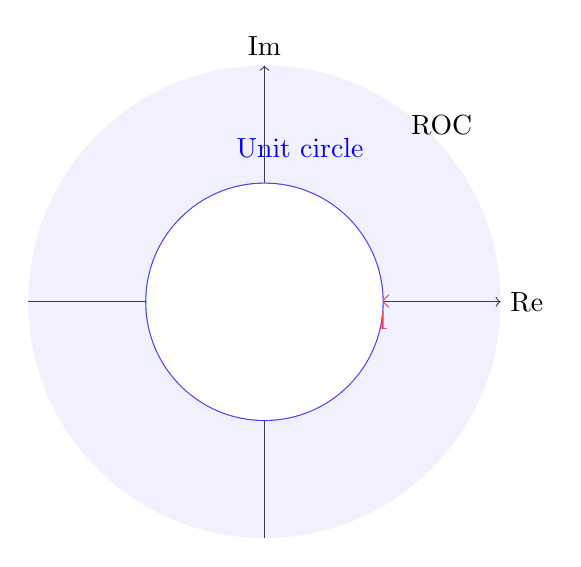
\begin{tikzpicture}[scale=1.5]
    \draw[->] (-2,0) -- (2,0) node[right] {Re};
    \draw[->] (0,-2) -- (0,2) node[above] {Im};
    \draw[thick,blue] (0,0) circle (1);
    \draw[red,thick] (0.6,0) node {$\times$} node[below] {$a$};
    \draw[red,thick] (1,0) node {$\times$} node[below] {$1$};
    \draw[green,thick] (0,0) node {$\circ$} node[below left] {$2$};
    \fill[blue!20,opacity=0.3] (0,0) circle (2);
    \fill[white] (0,0) circle (1);
    \node at (1.5,1.5) {ROC};
    \node at (0.3,1.3) [blue] {Unit circle};
\end{tikzpicture}
\end{center}

\vspace{0.3cm}
\textbf{Interpretation}:
\begin{itemize}
    \item As $n \to \infty$: $y[n] \to \frac{A}{1-a}$
    \item Time constant: $\tau = -1/\ln(a)$
\end{itemize}
\end{column}
\end{columns}
\end{frame}







\begin{frame}{Difference Equations and System Functions}
\textbf{General Difference Equation}:
\[
\sum_{k=0}^{N} a_k y[n-k] = \sum_{k=0}^{M} b_k x[n-k]
\]

% \vspace{0.3cm}
\textbf{Applying z-Transform}:
\begin{itemize}
    \item Use linearity and time-shifting properties
    \item Result: $\sum_{k=0}^{N} a_k z^{-k} Y(z) = \sum_{k=0}^{M} b_k z^{-k} X(z)$
\end{itemize}

% \vspace{0.3cm}
\textbf{System Function}:
\[
H(z) = \frac{Y(z)}{X(z)} = \frac{\sum_{k=0}^{M} b_k z^{-k}}{\sum_{k=0}^{N} a_k z^{-k}} = \frac{B(z)}{A(z)}
\]

% \vspace{0.3cm}
\textbf{Key Points}:
\begin{itemize}
    \item Numerator $\leftrightarrow$ input coefficients and delays
    \item Denominator $\leftrightarrow$ output coefficients and delays
    \item For causal system: ROC is $|z| > $ max pole magnitude
    \item Stable if all poles inside unit circle
\end{itemize}
\end{frame}



\begin{frame}{Example: First-Order System}
\textbf{Difference Equation}: $y[n] = ay[n-1] + x[n]$

\vspace{0.3cm}
\textbf{System Function} (by inspection):
\[
H(z) = \frac{1}{1 - az^{-1}}, \quad \text{ROC: } |z| > |a|
\]

% \vspace{0.3cm}
\textbf{Impulse Response}:
\[
h[n] = a^n u[n]
\]

\vspace{0.3cm}
% \textbf{Properties}:
\begin{itemize}
    \item Causal (ROC extends to $\infty$)
    \item Stable if $|a| < 1$ (pole inside unit circle)
    \item Frequency response (if stable): $H(e^{j\omega}) = \frac{1}{1 - ae^{-j\omega}}$
\end{itemize}

% \vspace{0.3cm}
\textbf{Three Methods to Find Output}:
\begin{enumerate}
    \item Iterate difference equation
    \item Convolve $x[n]$ with $h[n]$
    \item Use z-transforms and partial fractions 
\end{enumerate}
\end{frame}

\section{Summary}

\begin{frame}{Summary}
\textbf{z-Transform Properties}:
\begin{itemize}
    \item Provide powerful tools for signal and system analysis
    \item Transform complex operations (convolution) to simple ones (multiplication)
    \item Enable algebraic solution of difference equations
\end{itemize}

\vspace{0.3cm}
\textbf{LTI System Analysis}:
\begin{itemize}
    \item System function $H(z)$ completely characterizes LTI system
    \item Poles determine stability and transient behavior
    \item Zeros affect frequency response shape
    \item ROC determines causality and stability
\end{itemize}

\vspace{0.3cm}
\textbf{Key Relationships}:
\begin{itemize}
    \item Difference equation $\leftrightarrow$ Rational system function
    \item Impulse response $\leftrightarrow$ System function
    \item Convolution $\leftrightarrow$ Multiplication in z-domain
    \item Stability $\leftrightarrow$ Poles inside unit circle
\end{itemize}


\end{frame}

\end{document}